\documentclass{article}
\usepackage[utf8]{inputenc}
\usepackage[english]{babel}
\usepackage[]{amsthm} %lets us use \begin{proof}
\usepackage[]{amssymb} %gives us the character \varnothing
\usepackage{graphicx}
\usepackage{amsmath}
\usepackage[a4paper]{geometry}


\begin{titlepage}
    \begin{center}
        \vspace*{1cm}
            
        \Huge
        \textbf{Trabajo Práctico 2}
            
        \vspace{0.5cm}
        \LARGE
        \textbf{Aprendizaje Estadístico}
            
        \vspace{1.5cm}
            
        Ignacio Brusati - Federico Elías
            
        \vfill
            
        \vspace{0.8cm}
            
            
    \end{center}
\end{titlepage}


\begin{document}



\section{Introducción}
Se tiene un dataset con 62 muestras de tejido y para cada una de esas muestras contiene las expresiones de 2000 genes. Se desea clasificar en una de dos clases: normal o con tumor y hallar los genes más relevantes para clasificar. Los datos de este problema corresponden al artículo ‘Broad patterns of gene expression revealed by clustering of tumor and normal colon tissues probed by oligonucleotide arrays’ U. Alon, N. Barkai, D. A. Notterman, K. Gish, S. Ybarra, D. Mack, and A. J. Levine, Proc. Natl. Acad. Sci. USA, Vol. 96, Issue 12, 6745-6750, June 8, 1999.


\section{Normalización de los datos}
Dado que la mediana de los 62 tejidos varían enormemente y que tienen una relación lineal, lo primero que se realizó fue una normalización de los datos tomando logaritmo de todos los valores.\\

\noindent
Aquí se puede ver un histograma de las medianas con los datos originales:\\

\begin{center}
    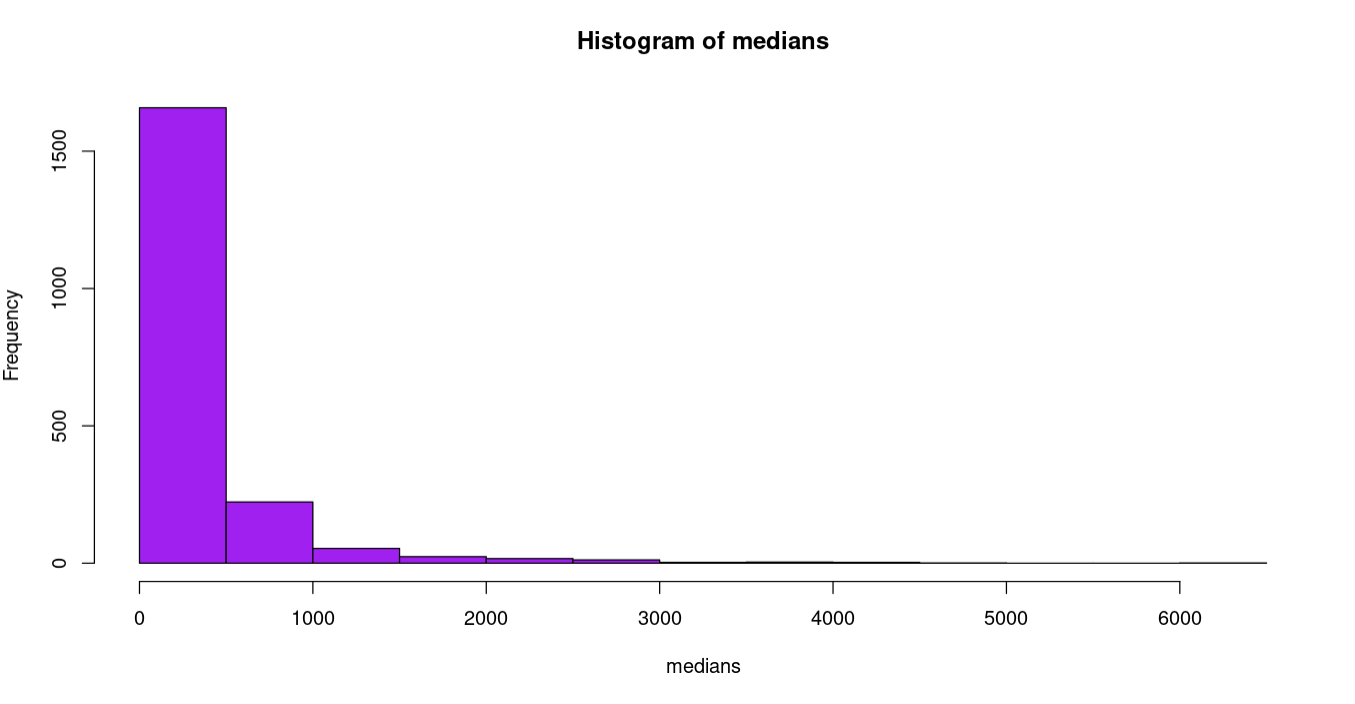
\includegraphics[width=1\textwidth]{img/medians.png}
\end{center}

\noindent
Aquí se puede observar un histograma de las medianas con los datos normalizados:\\

\begin{center}
    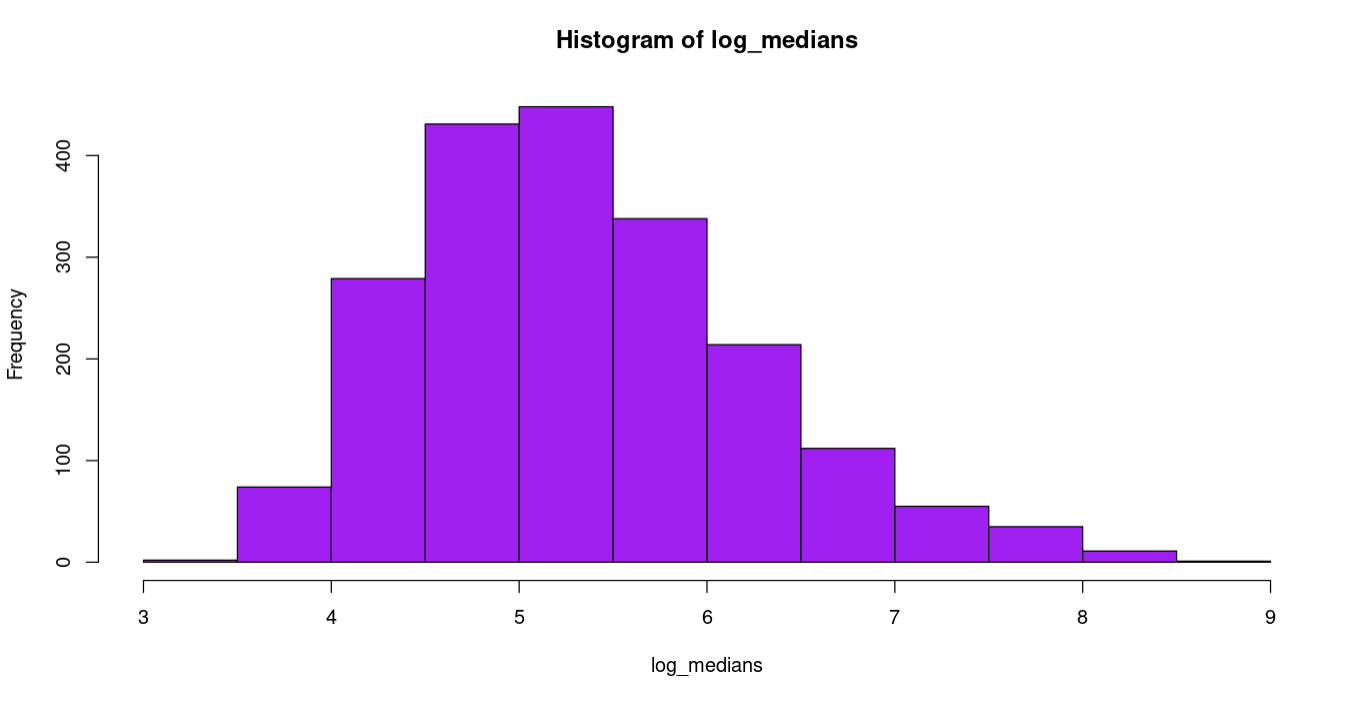
\includegraphics[width=1\textwidth]{img/log_medians.png}
\end{center}


\section{Árbol de clasificación y Bagging}
En primer lugar se realizó un árbol de decisión de clasificación. Como se puede ver a continuación, el árbol utiliza solamente los valores de 2 genes (el número 1671 y el número 548):\\

\begin{center}
    \includegraphics[width=1\textwidth]{img/árbol_común.png}
\end{center}

\noindent
El error de clasificación obtenido para este método fue $0.4176955$. A continuación se puede observar el gráfico de la curva ROC para este método:\\

\begin{center}
    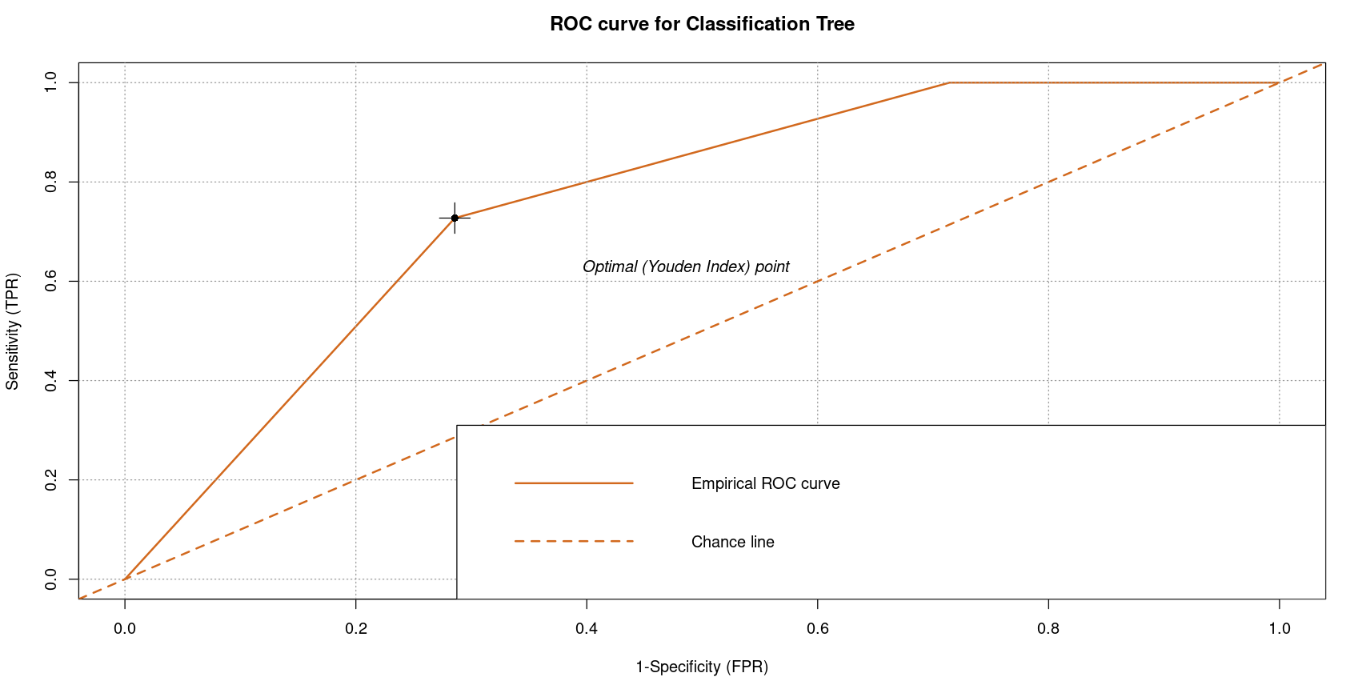
\includegraphics[width=1\textwidth]{img/roc_tree.png}
\end{center}

\noindent
El área bajo la curva ROC es 0.7597403.\\

\noindent
Luego, se utilizó el método de bagging. Este método propone utilizar diferentes muestras y construir un árbol para cada una de ellas. Para la clasificación de una nueva observación se utiliza el promedio de las clasificaciones de esos árboles. Las nuevas muestras se consiguen mediante bootstrap. Se realizó entonces un bagging con $15$ árboles y se puede ver que el error de clasificación disminuyó significativamente a $0.139266$.\\

\noindent
A continuación se puede observar el gráfico de la curva ROC para este método:\\

\begin{center}
    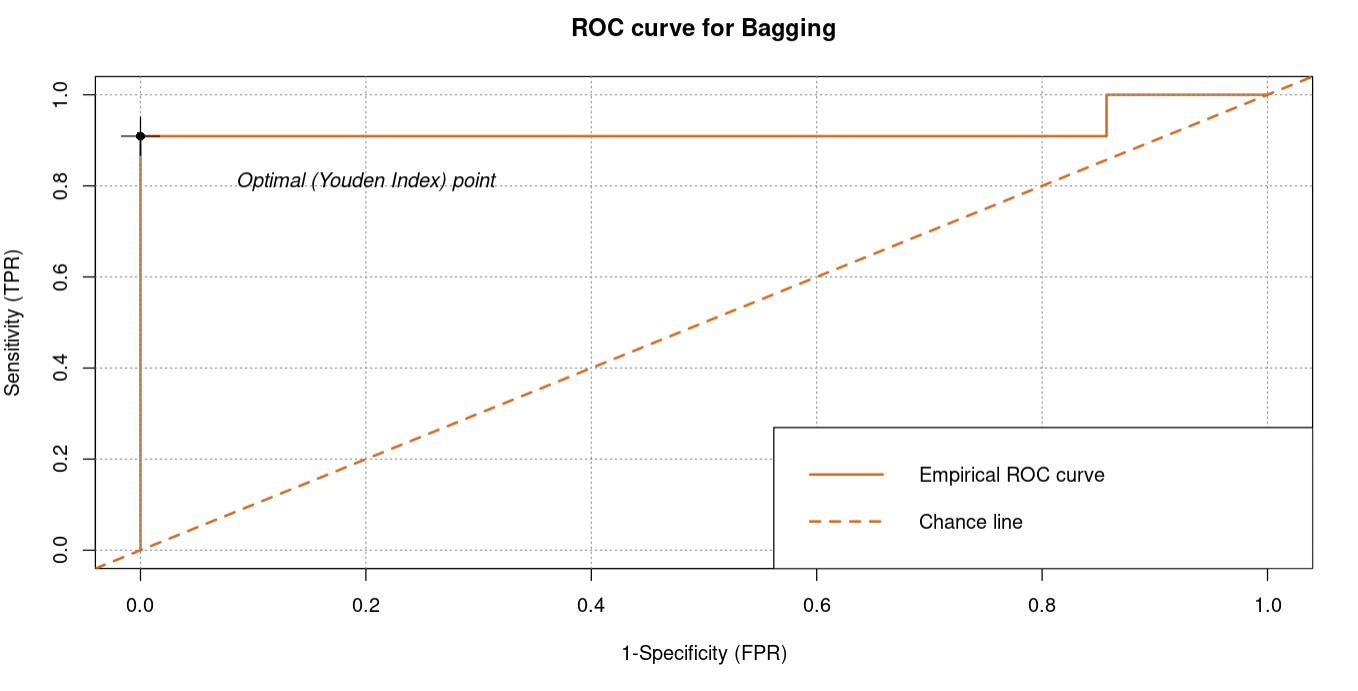
\includegraphics[width=1\textwidth]{img/roc_bagging.png}
\end{center}

\noindent
El área bajo la curva ROC es 0.9220779.\\


\section{Random Forest}
Este método propone que cada vez que se realiza una partición se elija al azar $m$ de las $p$ covariables disponibles con $m \approx \sqrt{p} $. De esta forma, se logra independizar a los estimadores buscando una mayor reducción en la varianza del estimador final.\\

\noindent
Se realizó la búsqueda del parámetro de cantidad de variables separadas aleatoriamente en cada partición para encontrar el óptimo. Se probaron todos los valores enteros entre 30 y 60 y el óptimo fue 38. A continuación se puede observar un gráfico con los diferentes valores probados y sus respectivos errores:\\

\begin{center}
    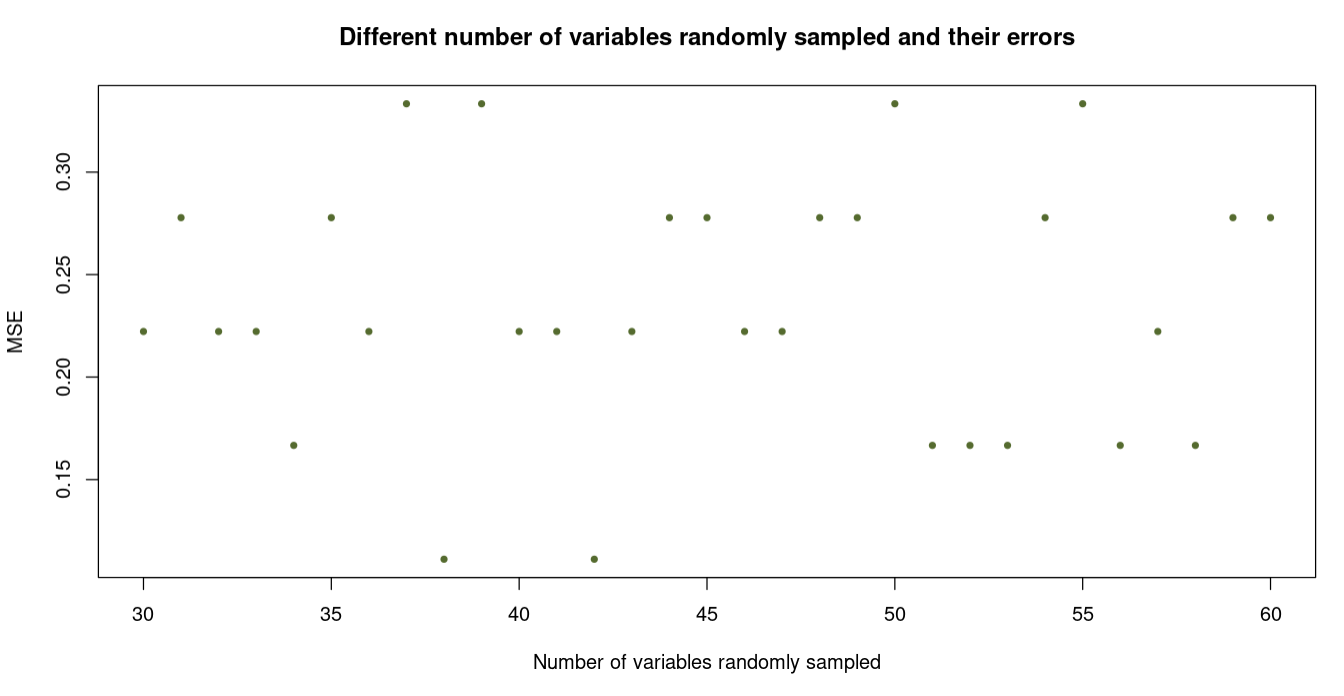
\includegraphics[width=1\textwidth]{img/hiper_rf.png}
\end{center}

\noindent
Usando el valor óptimo para la cantidad de variables separadas aleatoriamente el error de clasificación dio $0.1111111$, un valor cercano al error de clasificación de Bagging e incluso un poco menor.\\

\noindent
A continuación se puede observar el gráfico de la curva ROC para este método:\\

\begin{center}
    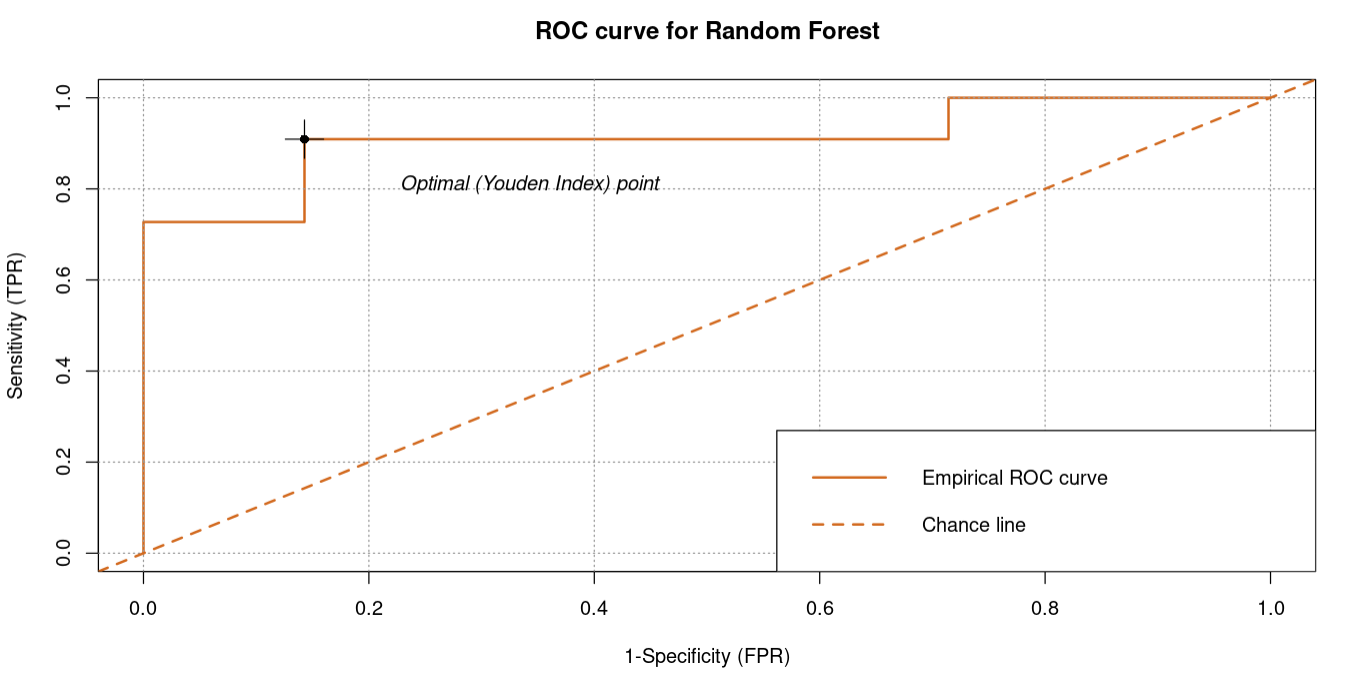
\includegraphics[width=1\textwidth]{img/roc_rf.png}
\end{center}

\noindent
El área bajo la curva ROC es 0.9090909.\\

\noindent
Se realizó también un gráfico de importancia de varibales. En el gráfico de la izquierda se puede visualizar la métrica Mean Decrease Accuracy (\text{\%IncMSE}) que representa el porcentaje en el que aumenta el error de clasificación si no se utilizara esa variable. De esta forma, a mayor valor de \text{\%IncMSE}, más importante es la variable. Por otro lado, a la derecha se grafica el Mean Decrease Gini (IncNodePurity) que es una medida de importancia de las variables que se basa en el índice de impureza de Gini que se utiliza para calcular las divisiones en los árboles. En este caso también, a mayor IncNodePurity, más importante la variable.\\

\begin{center}
    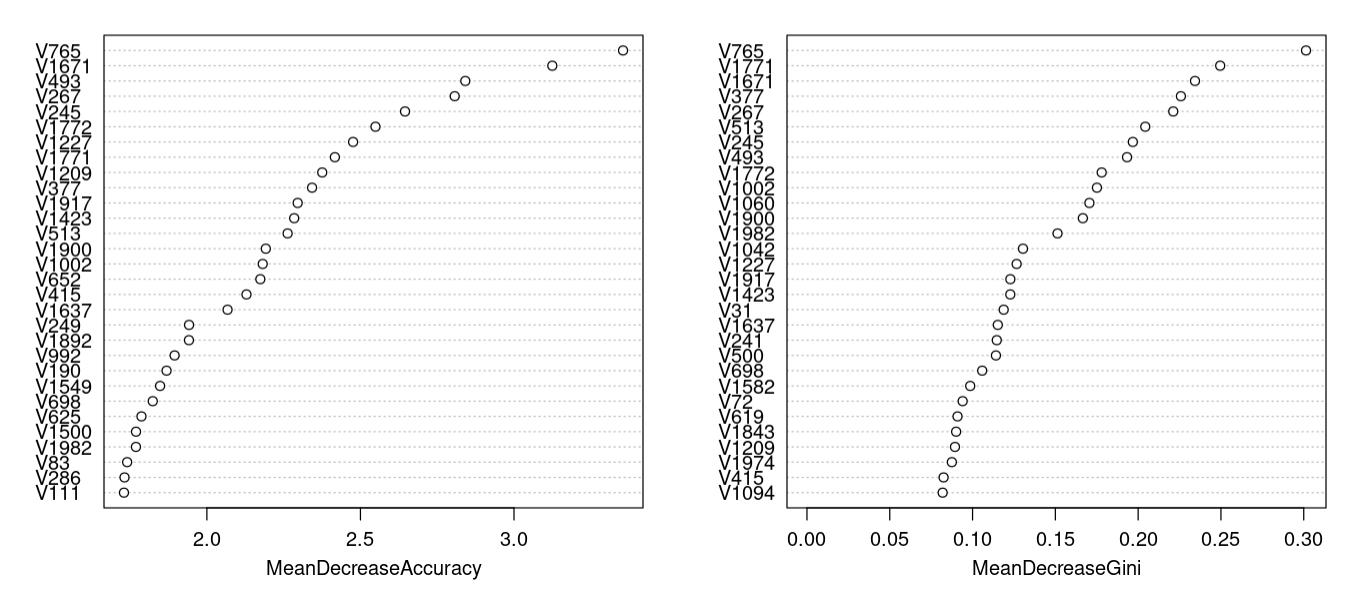
\includegraphics[width=1\textwidth]{img/rf_feature_importance.png}
\end{center}


\section{Boosting}
Se realizó la búsqueda del parámetro de cantidad de árboles usados para encontrar el óptimo. Se probaron un rango de valores entre 500 y 5000 con un salto de 500 y el óptimo fue 1000. A continuación se puede observar un gráfico con los diferentes valores probados y sus respectivos errores:\\

\begin{center}
    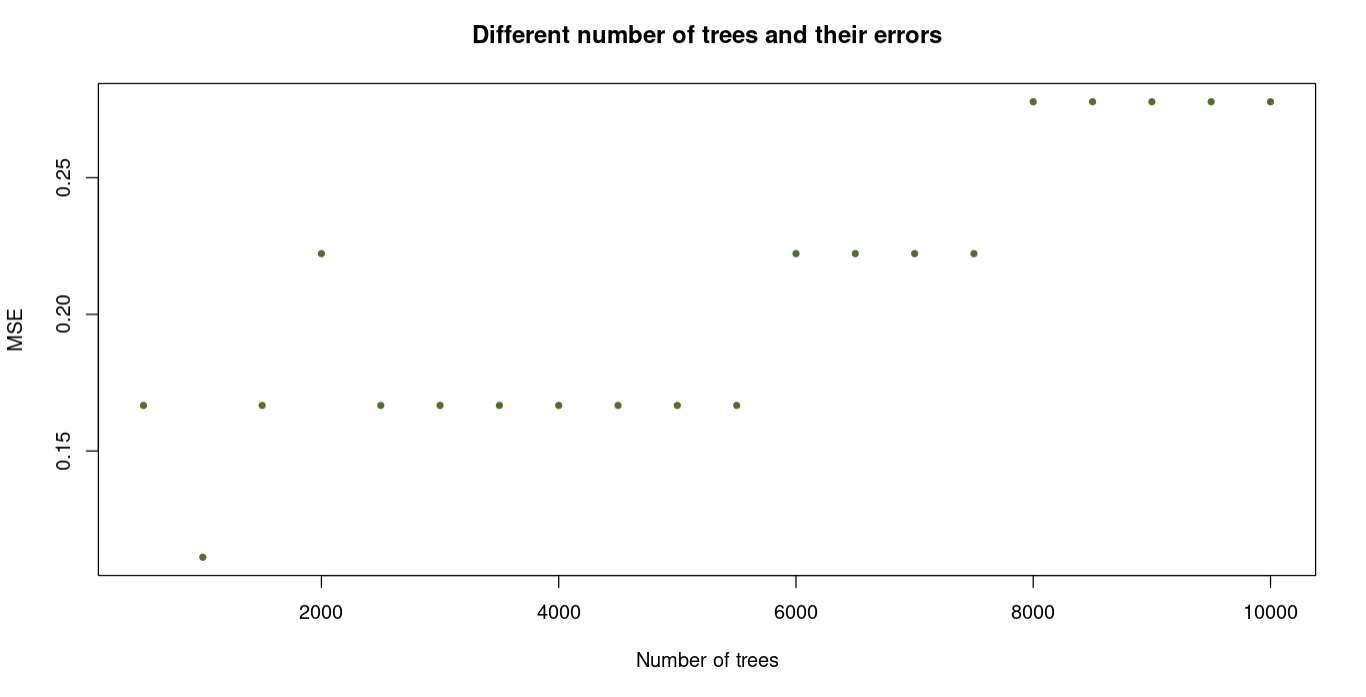
\includegraphics[width=1\textwidth]{img/hiper_boosting.png}
\end{center}

\noindent
A continuación se puede observar el gráfico de la curva ROC para este método:\\

\begin{center}
    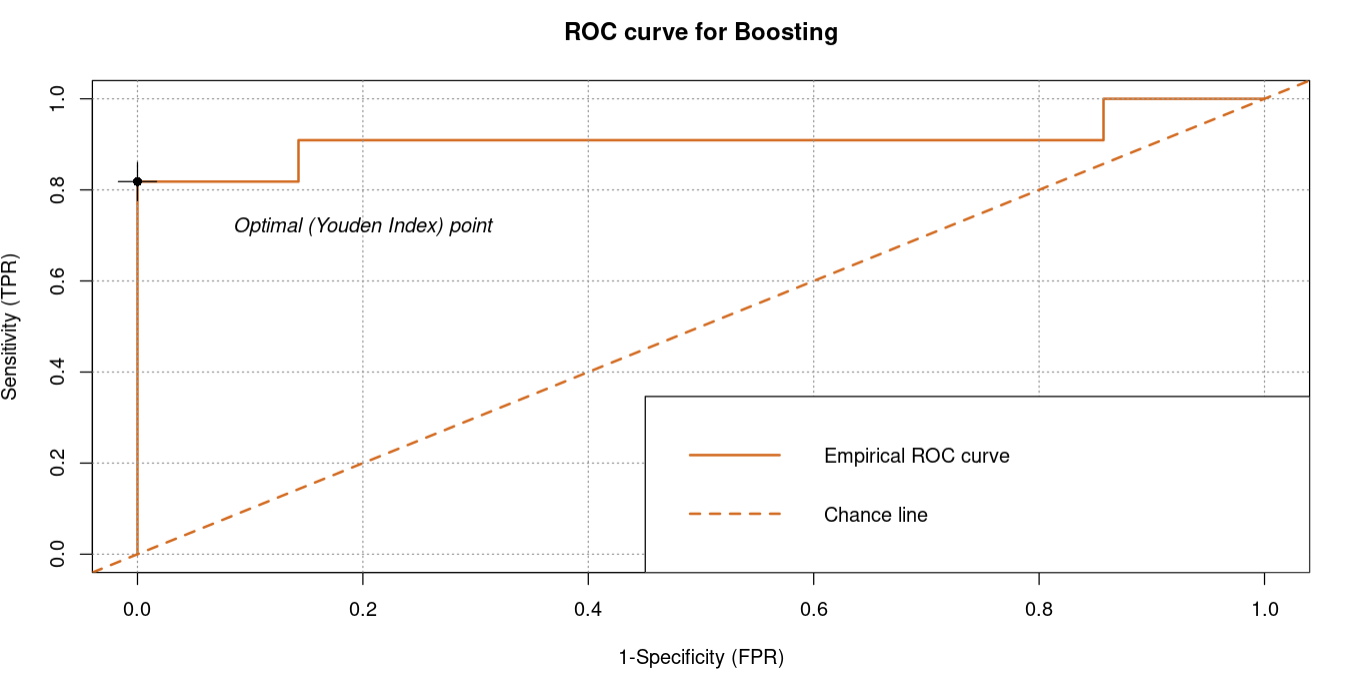
\includegraphics[width=1\textwidth]{img/roc_boosting.png}
\end{center}

\noindent
El área bajo la curva ROC es $0.9090909$ y el error de clasificación es $0.1111111$\\


\section{Nearest Shrunken Centroids}
El método Nearest Centroids calcula un centroide para cada gen para cada clase. El centroide se calcula como el valor promedio de un determinado gen en una determinada clase dividido por la desviación estándar dentro de la clase para ese gen. Así, al llegar una nueva observación, se toman los valores de esos genes y se los comparan con cada uno de estos centroides de clase. La clase cuyo centroide está más cerca es la clase predicha para esa nueva observación.\\

\noindent
Nearest Shrunken Centroids realiza una modificación al método recién descripto: los centroides calculados son reducidos en una cantidad llamada threshold. Esta reducción tiene dos ventajas. La primera tiene que ver con que puede mejorar la precisión de la clasificación ya que reduce el efecto de los genes 'ruidosos'. Por otra parte, este método es en sí una selección de genes ya que si al reducir el centroide de un gen este se hace 0 para todas las clases, entonces se puede no utilizar ese gen para predecir. Otra opción podría ser que el gen se hiciera 0 en una clase y en la otra no y eso indicaría que ese gen tiene una cierta incidencia en esa clase en particular que no se hace 0.\\

\noindent
Se realizó la búsqueda del parámetro de threshold. Se probaron un rango de valores entre 1 y 10 con un salto de 1 y el óptimo fue 2. A continuación se puede observar un gráfico con los diferentes valores probados y sus respectivos errores:\\

\begin{center}
    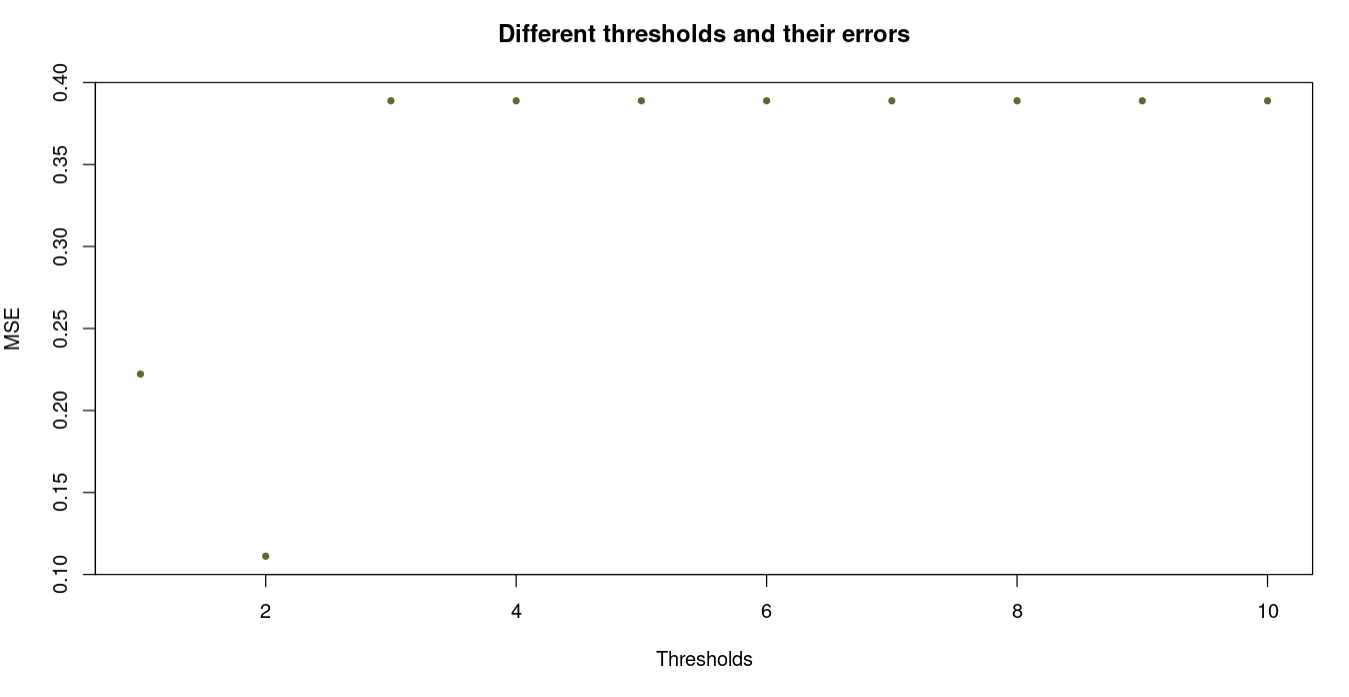
\includegraphics[width=1\textwidth]{img/hiper_nsc.png}
\end{center}

\noindent
A continuación se puede observar el gráfico de la curva ROC para este método:\\

\begin{center}
    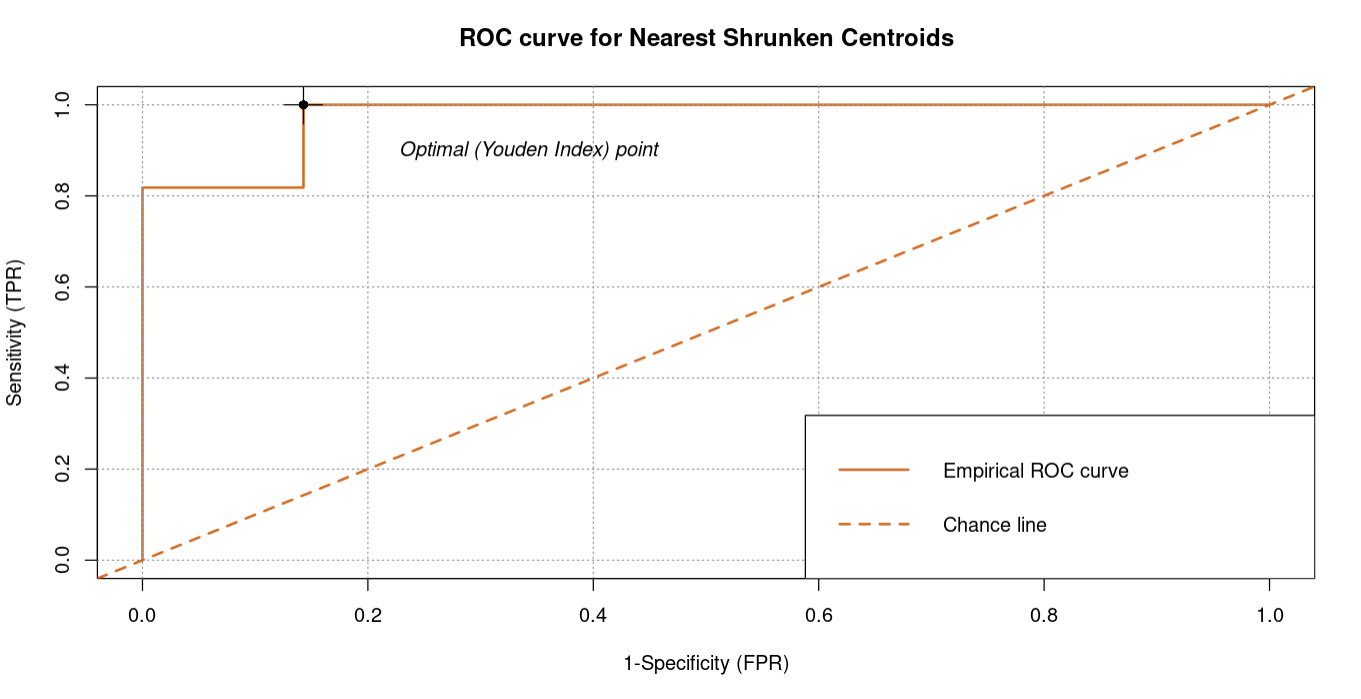
\includegraphics[width=1\textwidth]{img/roc_nsc.png}
\end{center}

\noindent
El área bajo la curva ROC es $0.974026$ y el error de clasificación es $0.1111111$. Como se puede ver, este método resultó ser muy bueno.\\

\noindent
Los genes más importantes para la predicción de la variable objetivo que no se hicieron 0 luego de aplicar el threshold resultaron ser: 1423, 1671, 493, 249, 765, 1042, 1900, 513, 1843, 897, 1772, 1730, 1771, 1494, 245, 822, 698, 625 1967, 377, 267, 1635, 138, 1810, 415. Para los métodos que siguen a continuación solamente se utilizaron estos genes.\\


\section{K-Nearest Neighbors (KNN)}
Se utilizó la distancia euclídea como métrica de distancia. Luego, se realizó un proceso de cross validation para obtener el valor de k óptimo. Para eso se utilizó un rango de valores de k entre 1 y 25 y el óptimo resultó ser un valor de $k=3$ vecinos. A continuación se puede observar un gráfico con los diferentes valores probados y sus respectivos errores:\\

\begin{center}
    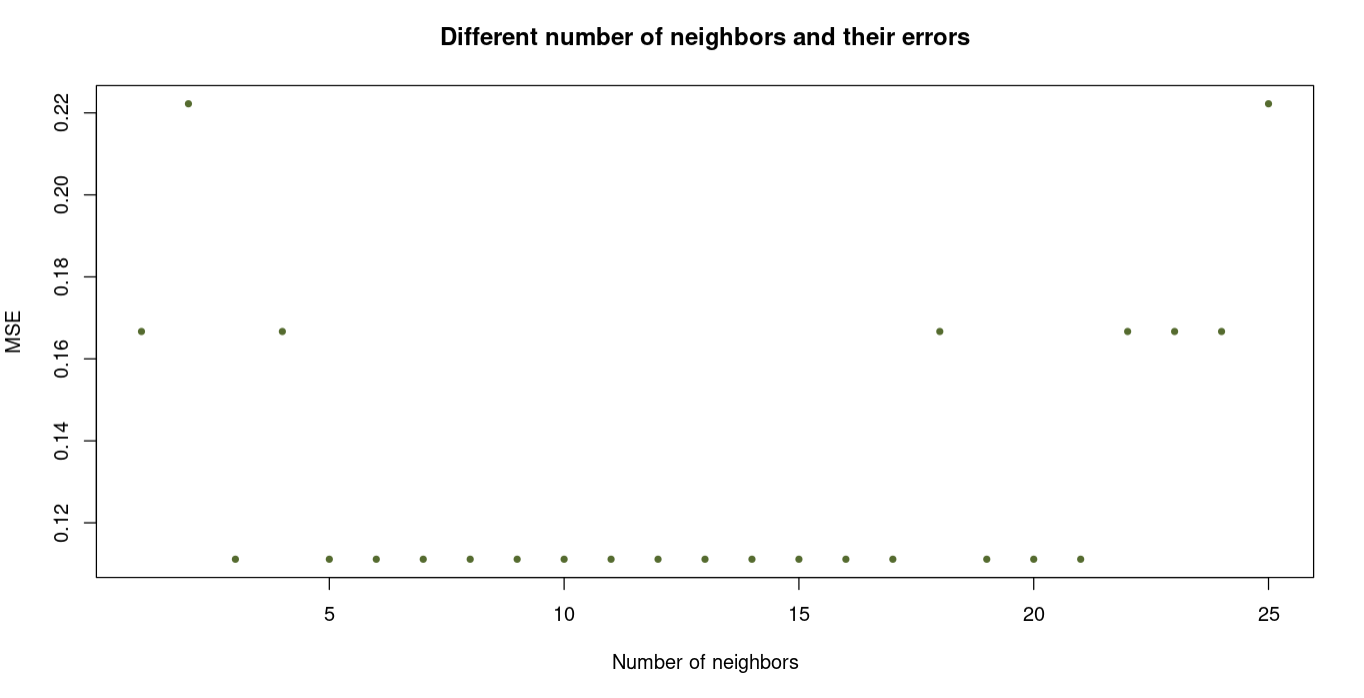
\includegraphics[width=1\textwidth]{img/hiper_knn.png}
\end{center}\\

\noindent
Usando el valor óptimo para la cantidad de vecinos el error de clasificación dio $0.1111111$.\\

\noindent
A continuación se puede observar el gráfico de la curva ROC para este método:\\

\begin{center}
    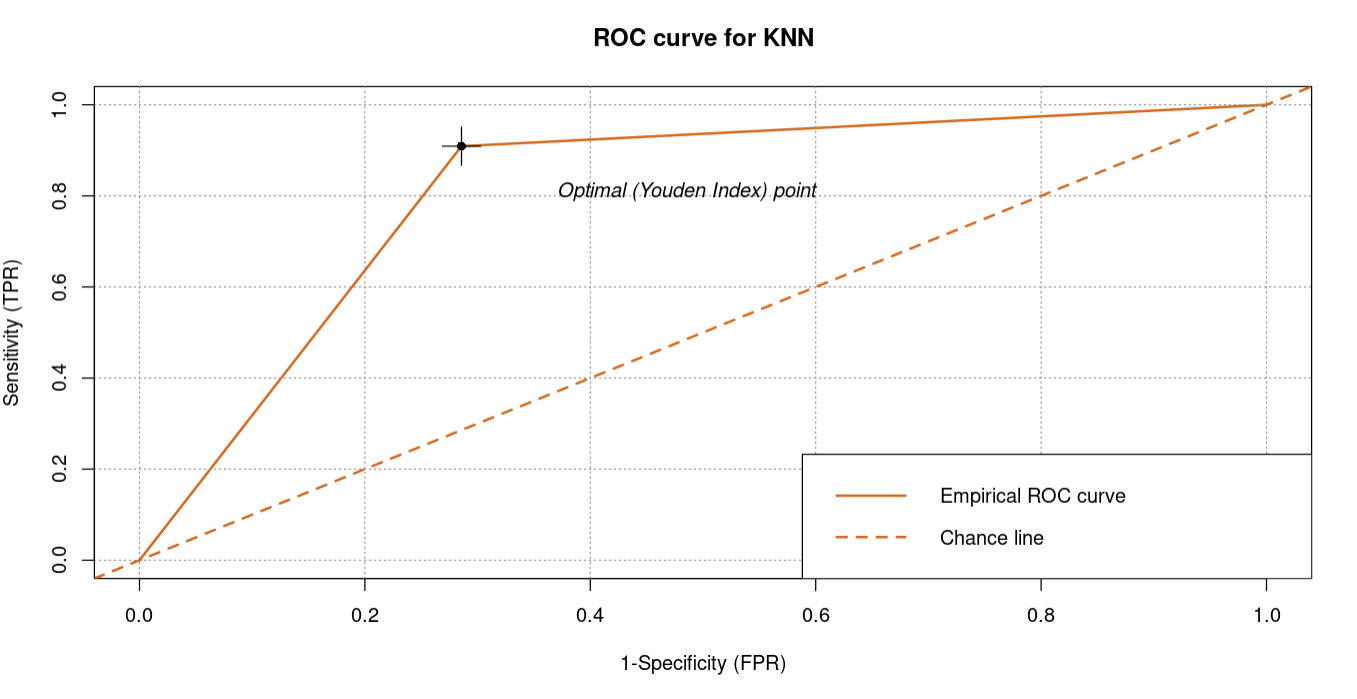
\includegraphics[width=1\textwidth]{img/roc_knn.png}
\end{center}

\noindent
El área bajo la curva ROC es $0.8116883$.\\


\section{Regresión Logística}
A continuación se puede observar el gráfico de la curva ROC para este método:\\

\begin{center}
    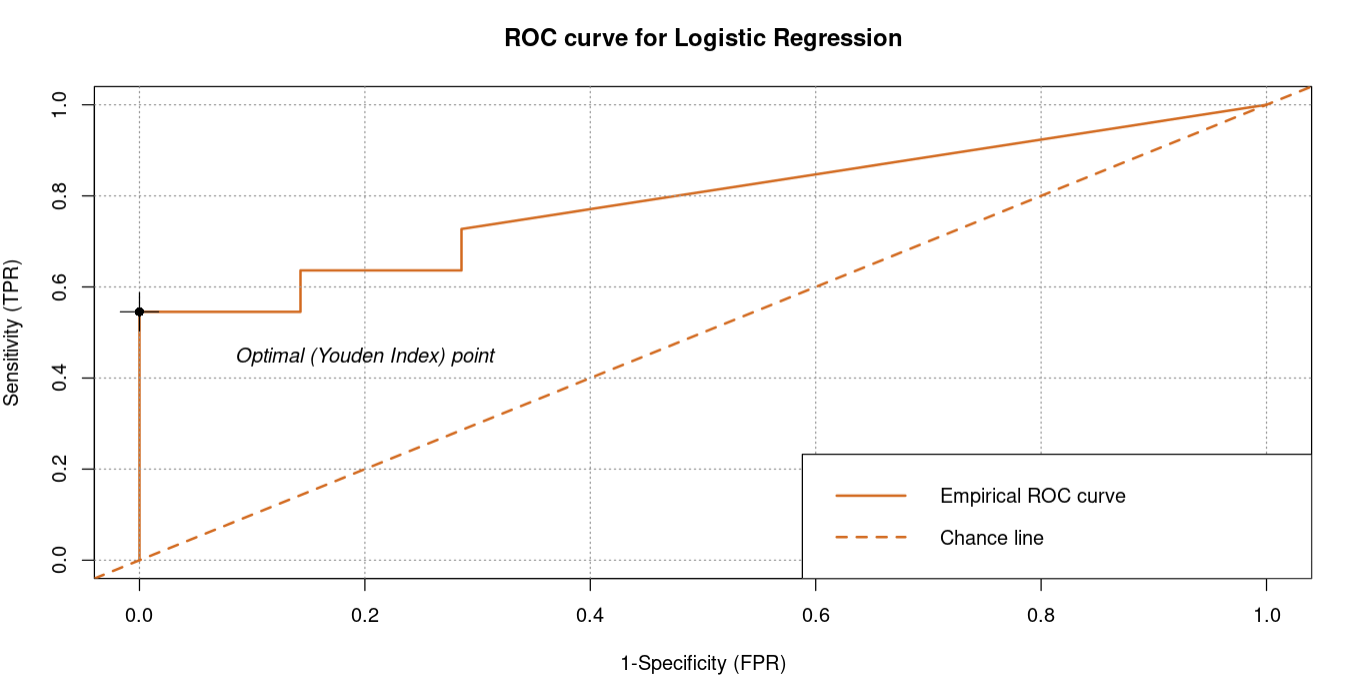
\includegraphics[width=1\textwidth]{img/roc_lr.png}
\end{center}

\noindent
El área bajo la curva ROC es $0.7857143$ y el error de clasificación es $0.3333333$\\


\section{Análisis Discriminante Lineal (LDA)}
Primero se verifica normalidad para las muestras pertenecientes a pacientes enfermos:
\begin{center}
    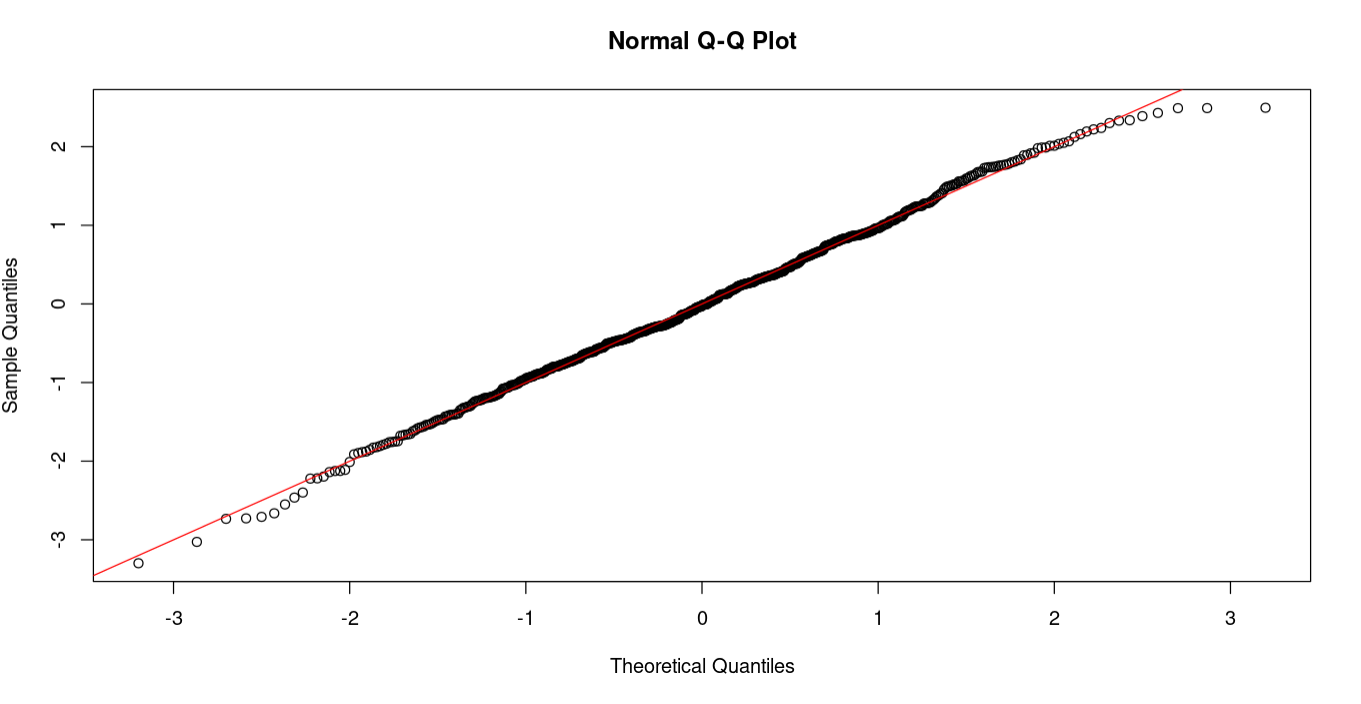
\includegraphics[width=1\textwidth]{img/qq_enfermos.png}
\end{center}

\noindent
Luego se verifica normalidad para las muestras pertenecientes a pacientes sanos:
\begin{center}
    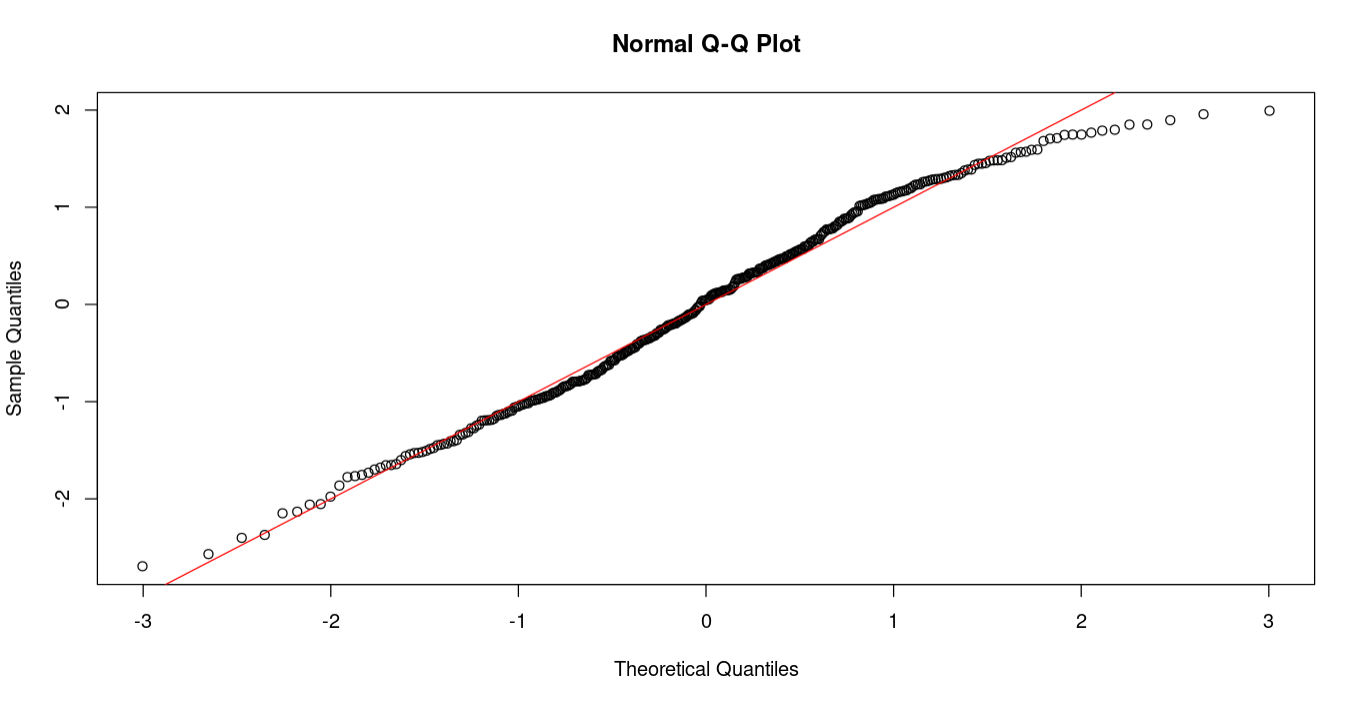
\includegraphics[width=1\textwidth]{img/qq_sanos.png}
\end{center}

\noindent
Se puede ver que ambas clases tienen una distribución que se puede aproximar a la Normal y por lo tanto se procede a realizar el análisis discriminante.\\

\noindent
Aquí se puede ver un histograma con las distribuciones de ambas clases:
\begin{center}
    \includegraphics[width=1\textwidth]{img/groups.png}
\end{center}

\noindent
Como se puede ver en el gráfico las clases tiene diferentes medias pero la varianza de la clase correspondiente a los pacientes enfermos es mayor que la varianza correspondiente a la clase de los pacientes sanos. Por lo tanto, dado que el método de LDA asume que las clases tienen la misma varianza, lo más probable es que este método no funcione bien para los datos que se tienen.\\

\noindent
A continuación se puede observar el gráfico de la curva ROC para este método:\\
\begin{center}
    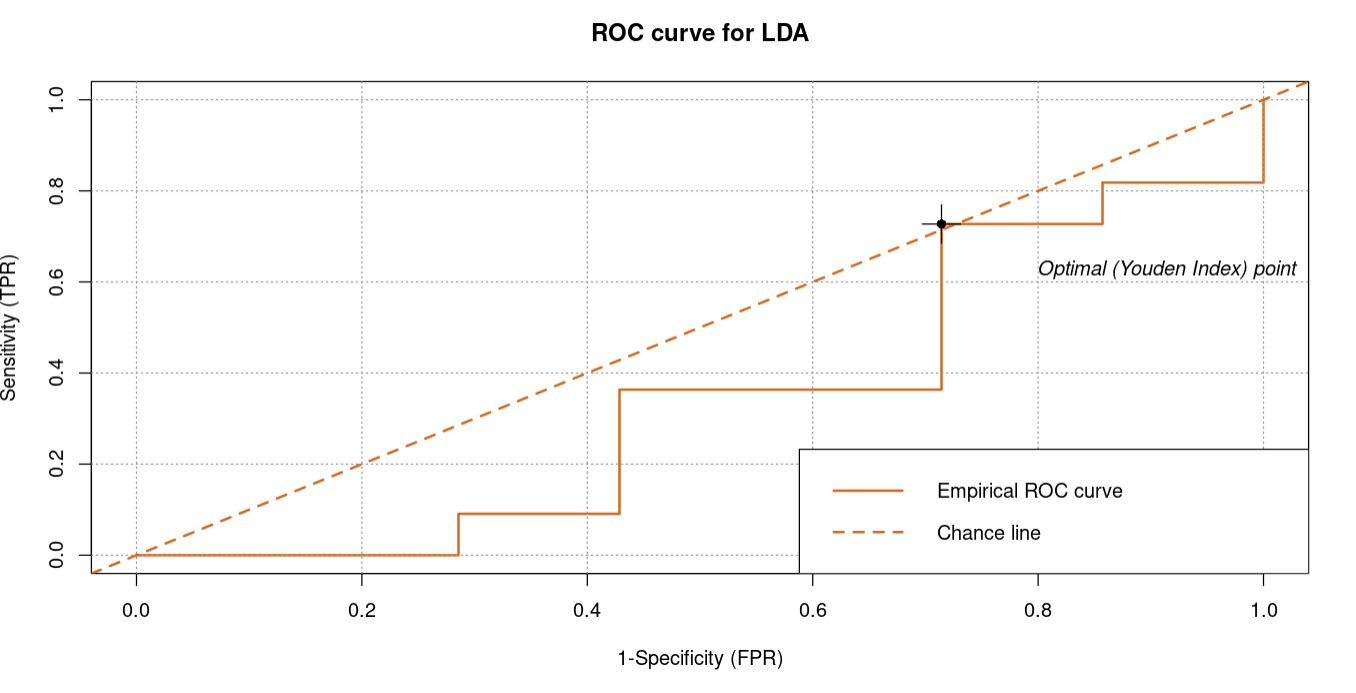
\includegraphics[width=1\textwidth]{img/roc_lda.png}
\end{center}

\noindent
El área bajo la curva ROC es $0.3376623$ y el error de clasificación es $0.4444444$. Efectivamente, el método resultó no ser bueno tal cual lo anteriormente comentado.


\section{Análisis Discriminante Cuadrático (QDA)}
De los 25 genes que fueron seleccionados por el método Nearest Shrunken Centroids se usaron 12. El error de clasificación fue 0.7222222 (peor que LDA) pero el área bajo la curva ROC fue 0.6103896 (mejor que LDA). Si bien el método mejora, sigue siendo bastante malo comparado con el resto de los métodos probados.

\begin{center}
    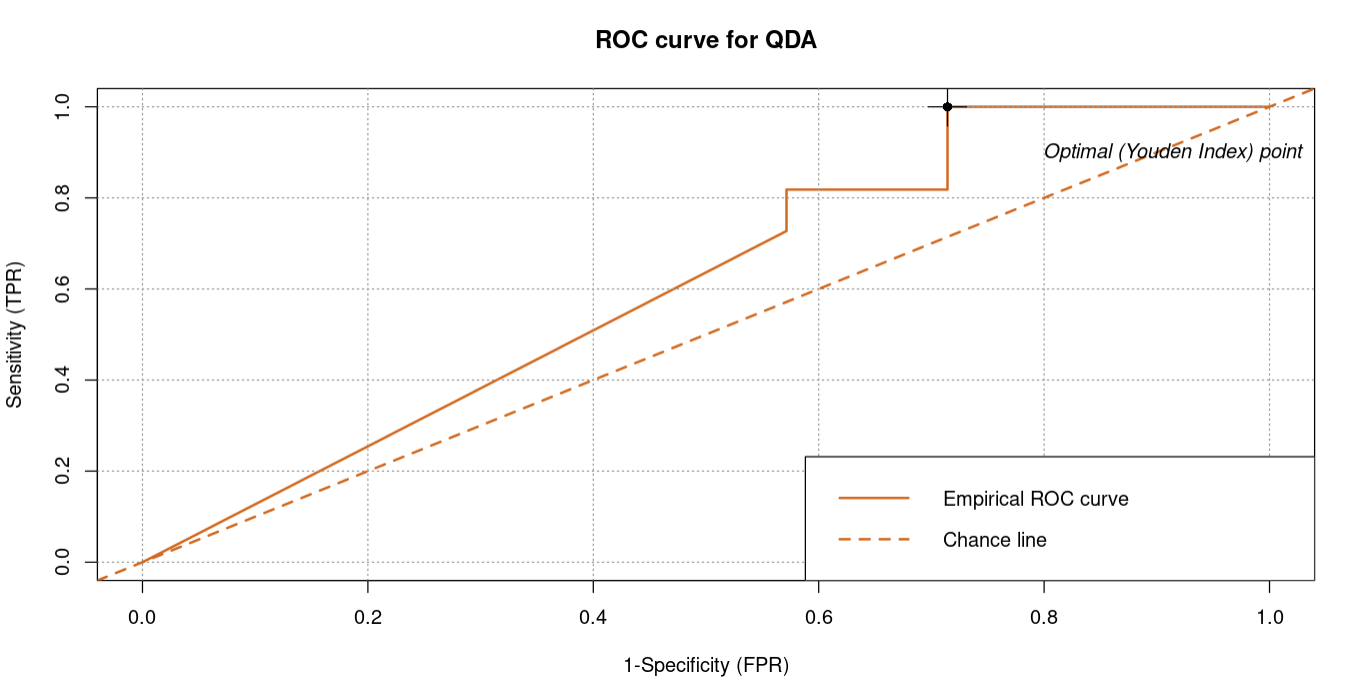
\includegraphics[width=1\textwidth]{img/roc_qda.png}
\end{center}


\section{Conclusión}
Luego de haber probado diferentes métodos de clasificación se puede decir que para los datos presentados el mejor método es el de Nearest Shrunken Centroids ya que es el que tiene un valor más alto de área bajo la curva ROC y el menor error de clasificación. Sin embargo, es importante destacar que los métodos basados en árboles (Bagging, Random Forest y Boosting) también obtuvieron muy buenos resultados en ambas métricas y podrían ser utilizados para clasificar.\\

\noindent
Por otro lado, se puede decir que los genes que fueron seleccionados por el método Nearest Shrunken Centroids son los más representativos a la hora de predecir a la variable objetivo. Además es importante destacar que la mayoría de esos genes también fueron seleccionados dentro del grupo de genes más importantes del método de Random Forest.


\end{document}